\subsection*{Metodo dei pacchetti d'onda}
Il metodo consiste nel far evolvere temporalmente un dato iniziale a pacchetto
d'onda nel potenziale stabilito e nel calcolare, dopo un opportuno tempo $t_0$,
la porzione di funzione d'onda che è oltre la barriera. Il tempo $t_0$ deve essere tale
da permettere il passaggio del pacchetto oltre la barriera, ma evitare riflessioni
ai bordi della scatola $[-L,L]$.
In tal caso, supponendo un pacchetto incidente da sinistra a destra,
il coefficiente di trasmissione sarà semplicemente
    $$ T = \frac{\int_b^L |\psi(x,t_0)|^2\mathrm d x}{\int_{-L}^L |\psi(x,t_0)|^2\mathrm d x} $$
Si vuole confrontare questo metodo con il metodo trovato al punto precedente,
per una barriera di potenziale di tipo gaussiano.\\
Essendo un pacchetto d'onda una sovrapposizione lineare di più onde stazionarie,
non possiede un momento ben definito. Il confronto verrà allora fatto tra il valor medio
del momento di un dato pacchetto, contro il corrispettivo autovalore
del metodo precedente (o quello che più gli si avvicina).
Si possono riscontrare le seguenti difficoltà:
\begin{itemize}
    \item pacchetti poco localizzati presentano problemi nella rilessione contro la barriera
    e nell'autointerferenza con i bordi della scatola
    \item pacchetti troppo localizzati presentano valori del momento
    molto dispersi a causa del principio di indeterminazione:
    questo introduce errori di approssimazione maggiori nel valutarne il valor medio
\end{itemize}
\bigskip
Di seguito i risultati.\\
\subsection*{Confronto dei due metodi}

\subsection*{Conclusioni}
Il metodo dei pacchetti d'onda non funziona con il potenziale a barriera quadrata
del punto 1, a causa della discontinuità del potenziale. La discontinuità
impedisce una buona riflessione del pacchetto d'onda incidente, risultando nella
permanenza di parte dell'onda nella zona della barriera per un lungo tempo.
Questo altera il calcolo dell'integrale della definizione di $T$ perchè
viene omessa una parte importante dell'onda. Il tempo che l'onda residua nella barriera
impiega a spegnersi è molto maggiore del tempo che il resto del pacchetto impiega
ad arrivare ai bordi della scatola e riflettersi, interagendo con sè stesso.
Il metodo risulta quindi inefficiente. Di seguito alcuni plot che mostrano
quanto detto.

% Metterle in un unico 'box' tutte e tre affiancate
\begin{figure}[h]
 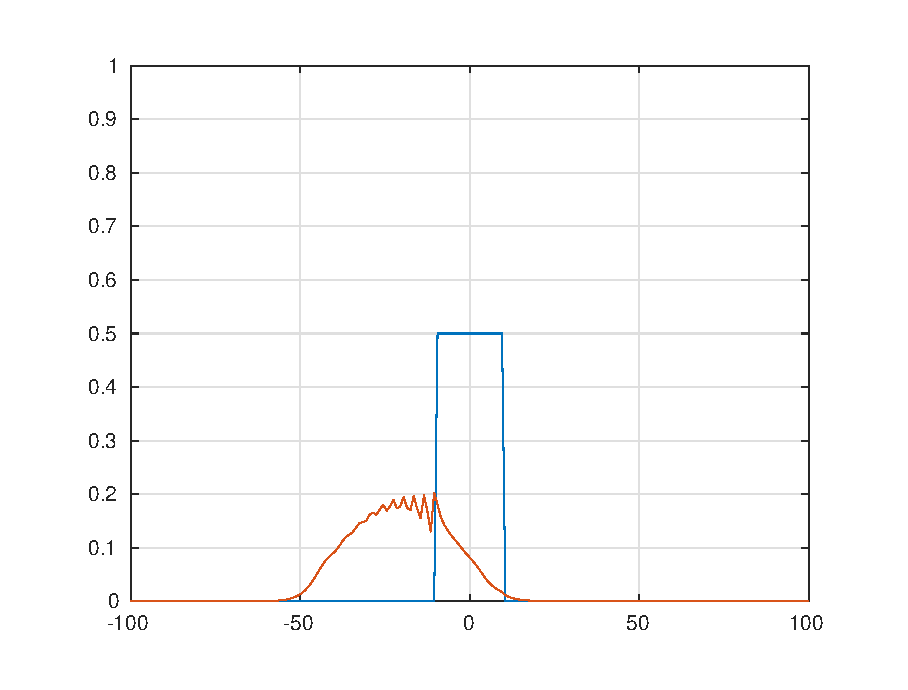
\includegraphics{square_transmission1.eps}
\end{figure}
\begin{figure}[h]
 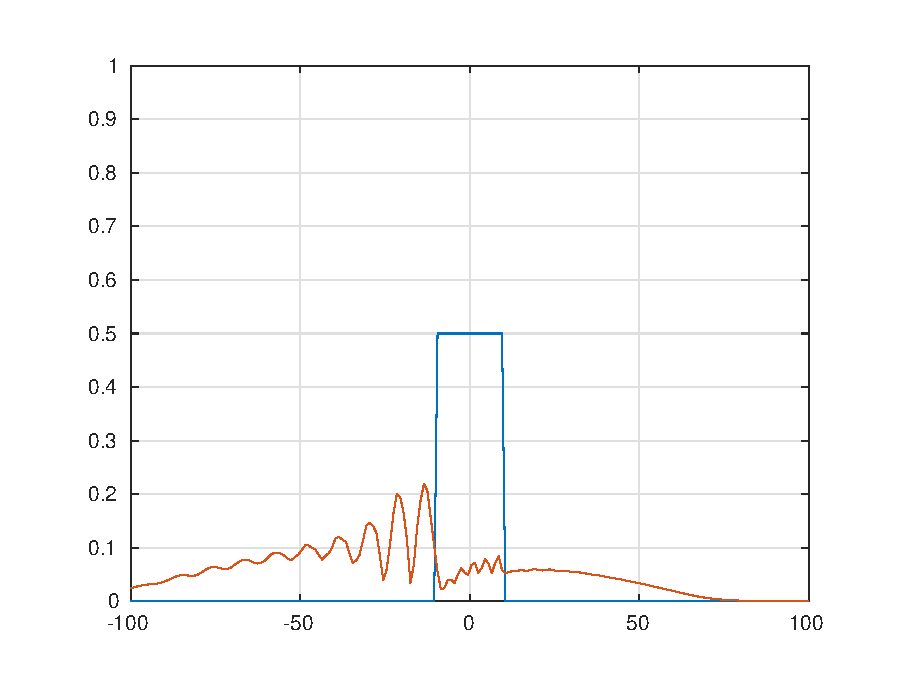
\includegraphics{square_transmission2.eps}
\end{figure}
\begin{figure}[h]
 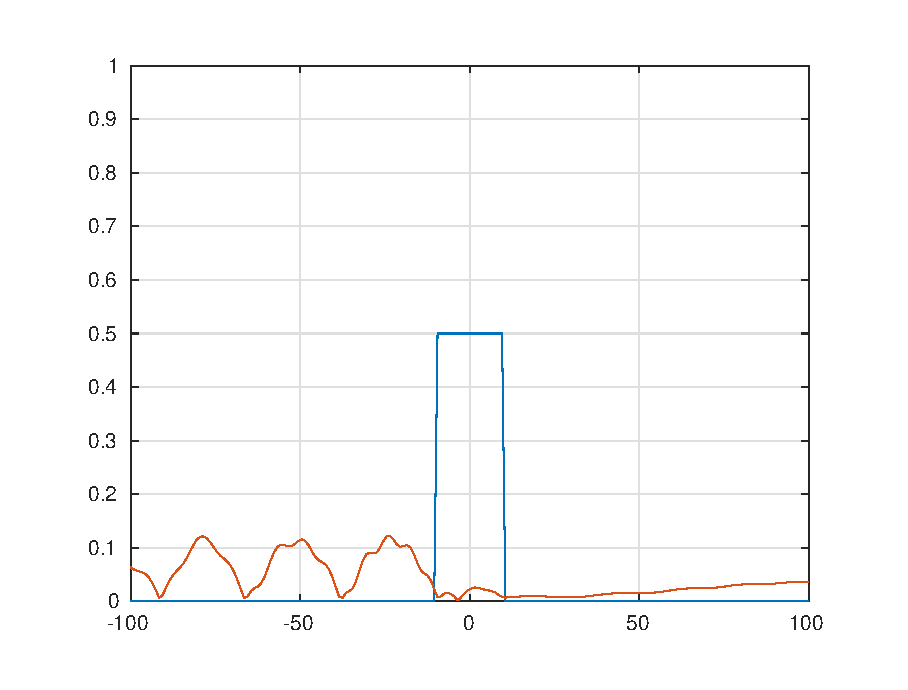
\includegraphics{square_transmission3.eps}
\end{figure}
